\documentclass[12pt]{article}
\usepackage[a5paper, margin=1cm, top=7mm]{geometry}
\usepackage{mathtools, tikz}
\usetikzlibrary{arrows.meta}
\tikzset{>={Stealth[scale=2]}}
\setlength\parindent{0mm}
\setlength\parskip{0mm}
\pagestyle{empty}

\begin{document}
\LARGE

\hfill
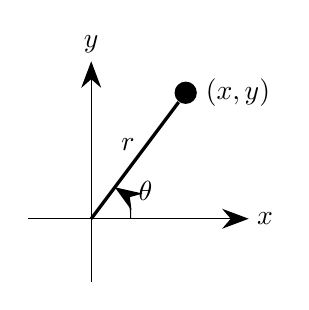
\begin{tikzpicture}[scale=2, inner sep=1mm]
\draw (1,0) edge[<-] (-.4,0) node[right] {$x$};
\draw (0,1) edge[<-]  (0,-.4) node[above] {$y$};
\node[label=right:{$(x,y)$}] (p) [circle, fill, scale=1] at (.6,.8) {};
\draw[very thick] (0,0) -- node[above left] {$r\!\!$}  (p);
\draw (.25,0) edge[bend right, ->] 
  node[above right, near start] {$\theta$} (.15,.2);
\end{tikzpicture}
\hfill
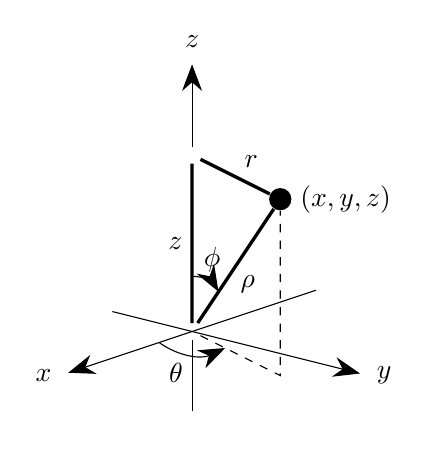
\begin{tikzpicture}[scale=0.28, inner sep=1mm]
\node (a) at (0,-4) {};
\node (b) at (0,0) {};
\node (c) at (0,8) {}; 
\node (d) at (0,11) {};
\node (e) at (0,12.5) {};
\node[label=right:{$(x,y,z)$}] (g) [circle, fill, scale=1] at (4,6) {};
\node (j) at (6,2) {};
\node (k) at (-6,-2) {};
\node (l) at (-4,1) {};
\node (m) at (8,-2) {};
\draw (-1.5,-.5) edge[bend right,->] node[below left] {$\theta$} (1.5,-.75);
\draw (0,2.5) edge[bend left,->] node[above] {$\,\,\phi$} (1.2,1.8);
\draw (a) -- (b); \draw (e) edge[<-] (c) node[above] {$z$};
\draw[very thick] (b) -- node[below right] {$\!\rho$} (g) 
  -- node[above right] {$r$} (c) -- node[left] {$z$} (b);
\draw (k) edge[<-] (j) node[left] {$x$};
\draw (m) edge[<-]  (l) node[right] {$y$};
\draw[dashed] (b) -- (4,-2) -- (g);
\end{tikzpicture}

\vfill
\textbf{Polar coordinates} {$(\theta,r)$}
\\[1mm] \textbf{Cylindrical coordinates} {$(\theta,r,z)$} 
\\[1mm] $x = r\cos\theta$
\qquad\qquad $dA = \pmb r\,d\theta\,dr$
\\ $y = r\sin\theta$
\qquad\qquad $dV = \pmb r\,d\theta\,dr\,dz$
\\ $z = z$
\\[4mm] $r$ = distance from $z$-axis = $\sqrt{x^2+y^2}$

\vfill
\vfill
\textbf{Spherical coordinates} {$(\theta,\rho,\phi)$}
\\[1mm] $x = \overbrace{\rho\sin\phi}^{\textstyle r} \cos\theta$
\\ $y = \rho\sin\phi \sin\theta$
\qquad $dV = \pmb{\rho^2\sin\phi} \,d\theta\,d\rho\,d\phi$
\\ $z = \rho\cos\phi$
\\[4mm] $\rho = {}$distance from origin${} = \sqrt{x^2+y^2+z^2}$
\\ $\phi = {}$angle with $z$-axis


\end{document}  
